\documentclass[11pt]{article}
\usepackage[utf8]{inputenc}
\usepackage[T1]{fontenc}
\usepackage{amsmath}
\usepackage{amssymb}
\usepackage{multicol}
\usepackage{geometry}
\usepackage{tikz}
\usepackage{enumitem}
\usepackage{xcolor}
\usepackage{titlesec}

% Configurações de layout
\geometry{a4paper, left=1cm, right=1cm, top=0.5cm, bottom=1.2cm}
\setlength{\columnseprule}{0.4pt}

% Cores para títulos
\titleformat{\section}{\normalfont\Large\bfseries\color{blue}}{\thesection}{1em}{}
\titleformat{\subsection}{\normalfont\large\bfseries\color{red}}{\thesubsection}{1em}{}

\title{\textcolor{orange}{Terceiro Trimestre: Matemática
    \\Progressão Geométrica - Revisão}}
\author{Professor: Jefferson}
\date{}

\begin{document}

\maketitle
\vspace{-1cm}

\begin{center}
\large{Nome: \underline{\hspace{8cm}} \quad Turma: \underline{\hspace{3cm}}}
\end{center}

\begin{multicols}{2}

\section*{Fórmulas Importantes}

\subsection*{Termo Geral da PG}

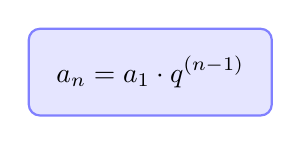
\begin{tikzpicture}
\node[rectangle, fill=blue!10, rounded corners, inner sep=10pt, draw=blue!50, thick] (box) {
$\displaystyle a_n = a_1 \cdot q^{(n-1)}$
};
\end{tikzpicture}

\textbf{Onde:}
\begin{itemize}
\item $a_n$ = termo que queremos
\item $a_1$ = primeiro termo
\item $n$ = posição do termo
\item $q$ = razão (quociente entre termos)
\end{itemize}

\subsection*{Razão da PG}

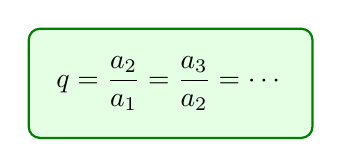
\begin{tikzpicture}
\node[rectangle, fill=green!10, rounded corners, inner sep=10pt, draw=green!50!black, thick] (box) {
$\displaystyle q = \frac{a_2}{a_1} = \frac{a_3}{a_2} = \cdots$
};
\end{tikzpicture}

\subsection*{Soma dos $n$ primeiros termos}

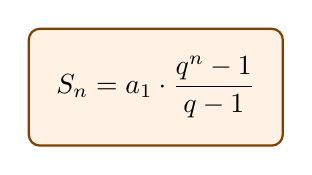
\begin{tikzpicture}
\node[rectangle, fill=orange!10, rounded corners, inner sep=10pt, draw=orange!50!black, thick] (box) {
$\displaystyle S_n = a_1 \cdot \frac{q^n - 1}{q - 1}$
};
\end{tikzpicture}

\section*{Exercícios Básicos}

\begin{enumerate}[leftmargin=*]

\item Determine a razão de cada PG:
\begin{enumerate}[label=\alph*)]
\item $(2, 6, 18, 54, \ldots)$
\item $(81, 27, 9, 3, \ldots)$
\item $(5, -10, 20, -40, \ldots)$
\end{enumerate}

\item Calcule o 5º termo de cada PG:
\begin{enumerate}[label=\alph*)]
\item $(3, 6, 12, 24, \ldots)$
\item $(256, 128, 64, 32, \ldots)$
\item $(1, 4, 16, 64, \ldots)$
\end{enumerate}

\item Encontre o 6º termo das PGs:
\begin{enumerate}[label=\alph*)]
\item $(2, 8, 32, 128, \ldots)$
\item $(1000, 100, 10, 1, \ldots)$
\end{enumerate}

\item Escreva os 4 primeiros termos da PG sabendo que:
\begin{enumerate}[label=\alph*)]
\item $a_1 = 2$ e $q = 3$
\item $a_1 = 64$ e $q = \frac{1}{2}$
\item $a_1 = 5$ e $q = -2$
\end{enumerate}

\item Calcule a soma dos:
\begin{enumerate}[label=\alph*)]
\item 5 primeiros termos da PG $(2, 6, 18, 54, \ldots)$
\item 6 primeiros termos da PG $(3, 12, 48, 192, \ldots)$
\item 4 primeiros termos da PG $(100, 50, 25, 12.5, \ldots)$
\end{enumerate}

\item Interpole 3 meios geométricos entre:
\begin{enumerate}[label=\alph*)]
\item 2 e 32
\item 3 e 48
\end{enumerate}

\item Problemas simples:
\begin{enumerate}[label=\alph*)]
\item Uma PG tem $a_1 = 2$ e $q = 4$. Qual é o 6º termo?
\item Uma PG tem $a_1 = 1000$ e $q = 0,1$. Qual é o 5º termo?
\item Calcule a soma dos 5 primeiros termos da PG $(1, 3, 9, 27, \ldots)$
\end{enumerate}

\item Complete as PGs:
\begin{enumerate}[label=\alph*)]
\item $( \_, 4, 8, 16, \_ )$
\item $(27, \_, 3, \_, \frac{1}{3})$
\item $( \_, 6, 18, 54, \_ )$
\end{enumerate}

\item Determine o número de termos das PGs:
\begin{enumerate}[label=\alph*)]
\item $(2, 6, 18, \ldots, 1458)$
\item $(1024, 512, 256, \ldots, 1)$
\end{enumerate}

\item Problemas do cotidiano:
\begin{enumerate}[label=\alph*)]
\item Uma população de bactérias dobra a cada hora. Se inicialmente há 100 bactérias, quantas haverá após 6 horas?
\item Uma bola é lançada de uma altura de 10m. A cada quique, ela sobe 70\% da altura anterior. Qual a altura do 5º quique?
\end{enumerate}

\end{multicols}

\end{document}
